\documentclass{article}

\usepackage{graphicx}

\title{Problem1 Report}
\author{Qi Liu}
\date{\today}

\begin{document}
	
\maketitle

\section{Original Figures}
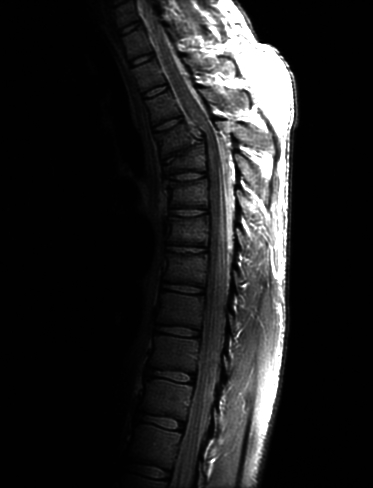
\includegraphics[width=0.5\textwidth]{../data/Fig1.jpg}
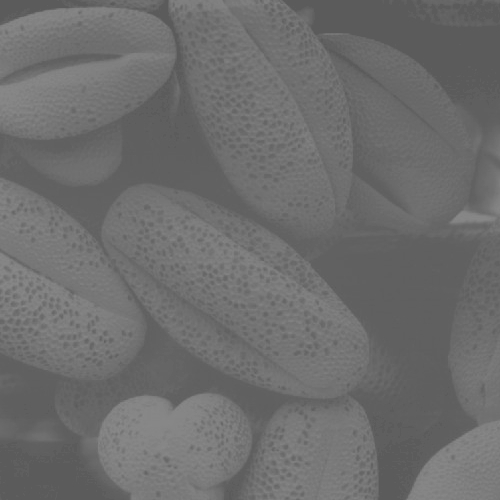
\includegraphics[width=0.5\textwidth]{../data/Fig2.jpg}
These two are the original figures. We can see that figure 1 is too dark and figure 2 is low-contrast. The below histograms show that.

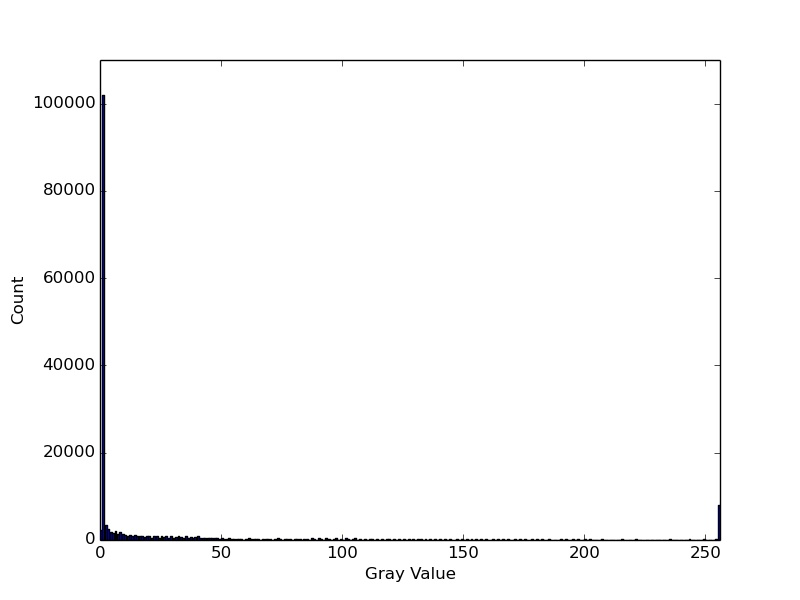
\includegraphics[width=0.5\textwidth]{../data/histogram_Fig1.jpg}
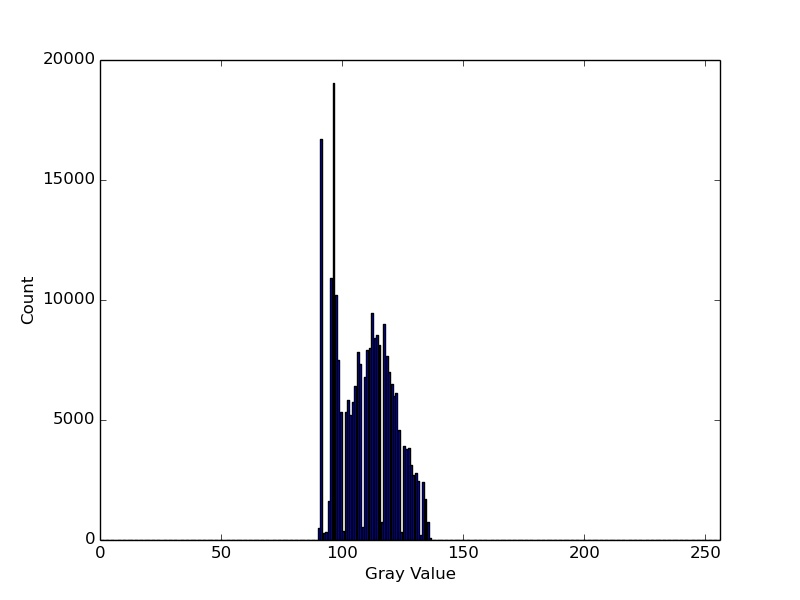
\includegraphics[width=0.5\textwidth]{../data/histogram_Fig2.jpg}
We can see that many pixels of figure 1 have very low gray level, thus figure 1 has many dark areas. About the second histogram, we can see the range of gray levels is very narrow, which means figure 2 is low-contrast.

\section{Histogram Equalization Figures}
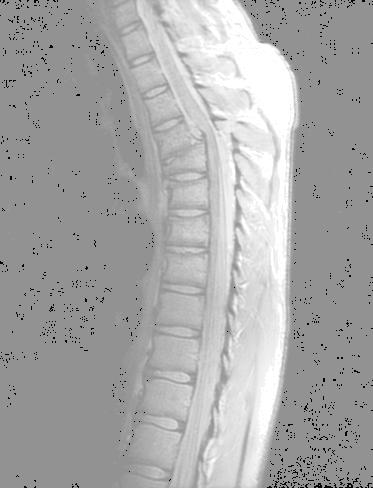
\includegraphics[width=0.5\textwidth]{../data/new_Fig1.jpg}
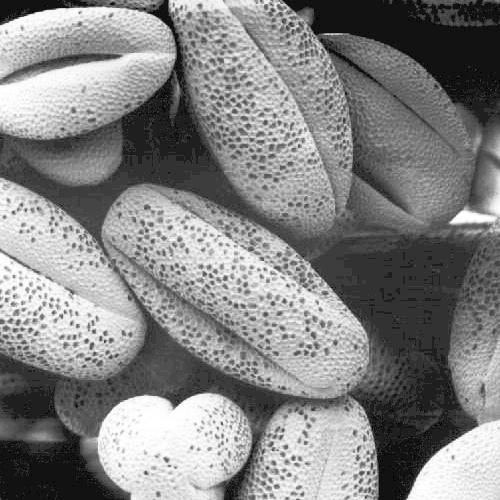
\includegraphics[width=0.5\textwidth]{../data/new_Fig2.jpg}
The figures above show the result after histogram equalization. We can see figure 2 is quite good but not figure 1. We can explain these by the following histograms.

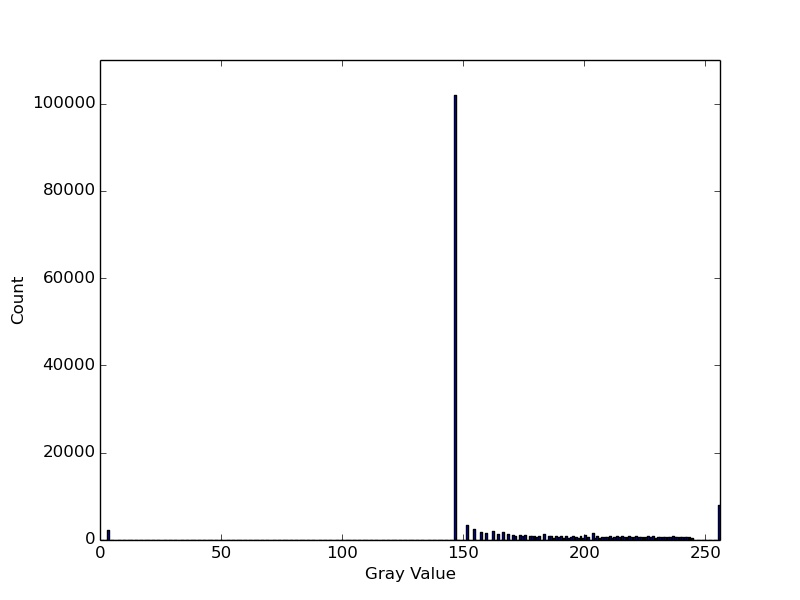
\includegraphics[width=0.5\textwidth]{../data/histogram_new_Fig1.jpg}
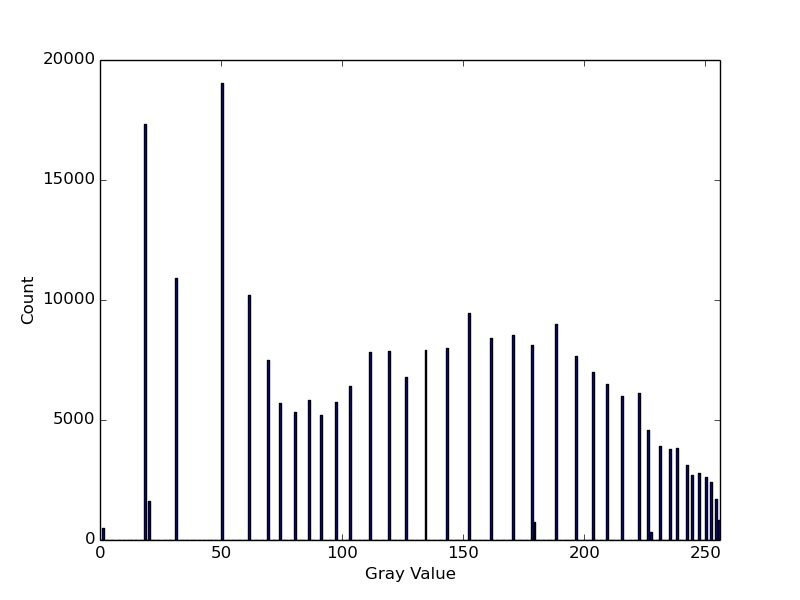
\includegraphics[width=0.5\textwidth]{../data/histogram_new_Fig2.jpg}
Since more that half pixels in figure 1 have gray level 0, we cannot split these pixels by only using histogram equalization, the first histogram shows that. And the second histogram is average, which indicates figure 2 is high-contrast after histogram equalization.

\end{document}